% Sections 6 and 7: data-efficiency curves (context) and labeled-budget thresholds (secondary result).

\section{Context: Data-Efficiency Curves}\label{sec:curves}

\subsection{How Much Domain Shift Reduces mAP (RQ1)}\label{sec:drop}

\begin{table*}[t]
\centering
\caption{Zero-shot drop relative to the source model on the source test set (0.342), and the gap remaining after the ceiling.}
\label{tab:drop}
\footnotesize
\setlength{\tabcolsep}{3pt}
\begin{tabular}{@{}lccccccc@{}}
\toprule
Shift & \mAPzero & Drop (95\% CI) & Relative drop & 3-epoch ceiling & Remaining gap & 12-epoch ceiling & Remaining gap \\
\midrule
lighting & 0.244 & 0.098 (0.092--0.106) & 28.8\% & 0.296 & 0.046 & 0.299 & 0.043 \\
weather  & 0.320 & 0.022 (0.012--0.032) & 6.5\%  & 0.336 & 0.007 & 0.331 & 0.011 \\
compound & 0.219 & 0.123 (0.112--0.133) & 35.9\% & 0.257 & 0.085 & 0.258 & 0.084 \\
\bottomrule
\end{tabular}
\tabnote{Remaining gap $= \mAPsrc - \text{ceiling}$. Ceilings are means over 2 seeds.}
\end{table*}

Table~\ref{tab:drop} gives the zero-shot drop of each shift and the gap that remains after each ceiling.

\textbf{Interaction.} $\mathrm{Drop}(\text{compound}) - \mathrm{Drop}(\text{lighting}) - \mathrm{Drop}(\text{weather}) = +0.002$ AP (CI $-0.012$ to $+0.016$). The point estimate is close to 0, but the test is weak: the CI half-width is 0.014 AP, equal to 63\% of the entire weather effect (0.022 AP); the smallest interaction detectable with 80\% power is 0.020 AP, that is, 91\% of the weather effect. The correct conclusion is: \textbf{these data cannot detect an interaction smaller than about 0.014--0.020 AP.} This is not evidence that the compound shift is additive.

\begin{table}[t]
\centering
\caption{Denominator of recovery (ceiling $-$ zero-shot).}
\label{tab:denom}
\footnotesize
\setlength{\tabcolsep}{3pt}
\begin{tabular}{@{}lcccc@{}}
\toprule
 & \multicolumn{2}{c}{3-epoch ceiling} & \multicolumn{2}{c}{12-epoch ceiling} \\
\cmidrule(lr){2-3}\cmidrule(lr){4-5}
Shift & Denominator & Multiple & Denominator & Multiple \\
 & (95\% CI) & of 0.01 & (95\% CI) & of 0.01 \\
\midrule
lighting & 0.052 (0.050--0.054) & 5.2 & 0.055 (0.053--0.058) & 5.5 \\
compound & 0.038 (0.034--0.042) & 3.8 & 0.038 (0.034--0.043) & 3.8 \\
weather  & 0.015 (0.012--0.018) & 1.5 & 0.011 (0.007--0.014) & 1.1 \\
\bottomrule
\end{tabular}
\end{table}

The weather denominator (Table~\ref{tab:denom}) is only one and a half times the minimum with the 3-epoch ceiling and sits close to the minimum with the 12-epoch ceiling. Per class (3-epoch ceiling): pedestrian 0.022, car 0.018, traffic light 0.013, traffic sign 0.009, so traffic sign is already below the minimum. In 1,000 bootstrap resamples, the denominator falls below the minimum 115 times for traffic light and 713 times for traffic sign.

\subsection{Recovery Curves (RQ2)}\label{sec:recovery}

\begin{table*}[t]
\centering
\caption{Recovery of reliable mAP against the 3-epoch ceiling (mean of 3 seeds, 95\% hierarchical bootstrap CI).}
\label{tab:recovery}
\footnotesize
\setlength{\tabcolsep}{3pt}
\begin{tabular}{@{}lccc@{}}
\toprule
$N$ & lighting & weather & compound \\
\midrule
10     & $-$1.17 ($-$1.23, $-$1.10) & $-$3.51 ($-$4.67, $-$2.71) & $-$1.33 ($-$1.59, $-$1.07) \\
25     & $-$0.78 ($-$0.83, $-$0.72) & $-$2.26 ($-$3.12, $-$1.60) & $-$0.90 ($-$1.11, $-$0.71) \\
50     & $-$0.36 ($-$0.43, $-$0.29) & $-$1.39 ($-$2.01, $-$0.96) & $-$0.36 ($-$0.49, $-$0.22) \\
100    & 0.01 ($-$0.03, 0.05)       & $-$0.42 ($-$0.85, $-$0.10) & 0.09 ($-$0.01, 0.20) \\
250    & 0.33 (0.28, 0.36)          & 0.22 (0.05, 0.35)          & 0.52 (0.46, 0.58) \\
500    & 0.44 (0.41, 0.46)          & 0.50 (0.39, 0.60)          & 0.66 (0.61, 0.71) \\
1,000  & 0.55 (0.52, 0.57)          & 0.77 (0.66, 0.86)          & 0.87 (0.82, 0.91) \\
2,000  & 0.66 (0.63, 0.69)          &                            & \\
5,000  & 0.80 (0.78, 0.82)          &                            & \\
10,000 & 0.91 (0.89, 0.93)          &                            & \\
full pool & 1 (18,015 images)       & 1 (1,985 images)           & 1 (1,738 images) \\
\bottomrule
\end{tabular}
\end{table*}

\textbf{At small $N$, fine-tuning makes the model worse than zero-shot.} Recovery is negative at $N \leq 50$ in all three shifts, and at $N = 100$ for weather (Table~\ref{tab:recovery}, Fig.~\ref{fig:rec-lighting}). The cause is the fixed schedule: 10 images receive 500 updates, that is, about 100 epochs. This is exactly the region where \aldi has its largest advantage, and Section~\ref{sec:decomp} shows that most of that advantage is due to FT overfitting. At large $N$, source forgetting also rises again (Section~\ref{sec:secondary}).

\begin{figure}[t]
\centering
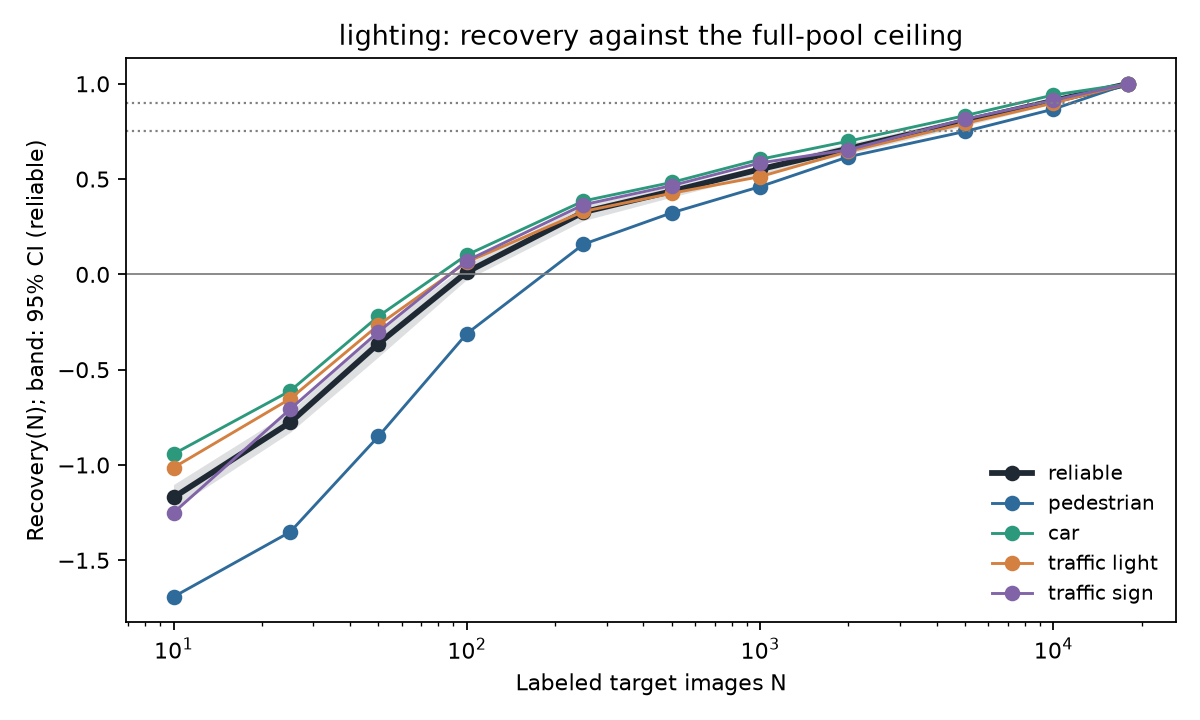
\includegraphics[width=\columnwidth]{recovery_lighting.png}
\caption{Lighting: recovery against the 3-epoch ceiling (mean of 3 seeds), for reliable mAP and for each class; the gray band is the 95\% CI of reliable mAP. The two dotted lines mark the 0.75 and 0.90 levels.}
\label{fig:rec-lighting}
\end{figure}

\begin{table}[t]
\centering
\caption{Per-class recovery at $N = 1{,}000$, 3-epoch ceiling.}
\label{tab:perclass}
\footnotesize
\setlength{\tabcolsep}{3pt}
\begin{tabular}{@{}lcccc@{}}
\toprule
Shift & pedestrian & car & traffic light & traffic sign \\
\midrule
lighting & 0.46 & 0.60 & 0.51 & 0.58 \\
weather  & 0.82 & 0.82 & \begin{tabular}[t]{@{}c@{}}undetermined\\(105/1,000)\end{tabular} & undetermined \\
compound & \begin{tabular}[t]{@{}c@{}}undetermined\\(120/1,000)\end{tabular} & 0.88 & 0.88 & 0.82 \\
\bottomrule
\end{tabular}
\end{table}

On lighting, against the 3-epoch ceiling, pedestrian recovers slowest (0.46; Table~\ref{tab:perclass}). Against the 12-epoch ceiling, traffic light is slowest (0.44) and pedestrian reaches 0.54 (0.40, 0.69), because 12 epochs raise the traffic light ceiling and lower the pedestrian ceiling. The ordering of the classes therefore depends on the ceiling, and it is not enough to separate re-learning the class distribution from learning new visual features. On compound and weather, the classes that can still be cited track each other closely.

\subsection{12-Epoch versus 3-Epoch Ceiling}\label{sec:ceiling12}

If the 3-epoch ceiling were undertrained, the recovery denominator would be small, recovery would be inflated, and every threshold would be a lower bound on the true requirement. The 12-epoch ceiling was run to test this. The rule, written before scoring: the 12-epoch ceiling replaces the 3-epoch ceiling as the denominator \textbf{regardless of the outcome}; ``materially higher'' means a paired difference $\geq 0.005$ AP with the lower CI bound above 0; both threshold tables are reported.

\begin{table*}[t]
\centering
\caption{12-epoch versus 3-epoch ceiling (reliable mAP, mean of 2 seeds, paired difference).}
\label{tab:ceil}
\footnotesize
\setlength{\tabcolsep}{3pt}
\begin{tabular}{@{}llcccc@{}}
\toprule
Shift & Pool & 3-epoch ceiling & 12-epoch ceiling & 12 $-$ 3 epochs (95\% CI) & Materially higher? \\
\midrule
lighting & full pool (18,015) & 0.2960 & 0.2989 & $+$0.0029 ($+$0.0014, $+$0.0041) & no \\
lighting & 1,738              & 0.2777 & 0.2756 & $-$0.0021 ($-$0.0031, $-$0.0007) & no \\
weather  & full pool (1,985)  & 0.3355 & 0.3310 & $-$0.0045 ($-$0.0067, $-$0.0025) & no \\
weather  & 1,738              & 0.3344 & 0.3300 & $-$0.0044 ($-$0.0067, $-$0.0022) & no \\
compound & full pool (1,738)  & 0.2572 & 0.2578 & $+$0.0005 ($-$0.0021, $+$0.0037) & no \\
\bottomrule
\end{tabular}
\end{table*}

\begin{itemize}
\item \textbf{No ceiling is materially higher} (Table~\ref{tab:ceil}). On the lighting full pool, 12 epochs exceed 3 epochs by 0.003 AP: statistically significant, but below the preset level of 0.005.
\item \textbf{On the small pools, 12 epochs either do not help or make things worse.} Compound is unchanged; weather and the 1,738-image lighting pool drop by 0.0021--0.0045 AP. This is consistent with 12 epochs starting to overfit at this pool size, but it has not been verified, and compound (also 1,738 images) does not drop.
\item Per class, only traffic light ($+0.0077$) and traffic sign ($+0.0053$) on the lighting full pool are materially higher.
\item Source forgetting is heavier at 12 epochs: $-0.043$ / $-0.015$ / $-0.032$ AP on the source test set (lighting / weather / compound), against $-0.026$ / $-0.005$ / $-0.018$ for the 3-epoch ceiling.
\end{itemize}

Per the rule, \mAPc is the 12-epoch ceiling: 0.2989 / 0.3310 / 0.2578. With this ceiling, the 3-epoch full-pool run becomes the top rung of the ladder and is a measurement, no longer equal to 1 by definition (Table~\ref{tab:rec2}, Figs.~\ref{fig:rec-lighting-e12} and~\ref{fig:rec-compound-e12}). Both ceilings are presented side by side; neither is chosen as better after the results have been seen.

\begin{table*}[t]
\centering
\caption{Recovery against the two ceilings (seed mean, 95\% CI).}
\label{tab:rec2}
\footnotesize
\setlength{\tabcolsep}{3pt}
\begin{tabular}{@{}lcccc@{}}
\toprule
 & \multicolumn{2}{c}{lighting} & \multicolumn{2}{c}{compound} \\
\cmidrule(lr){2-3}\cmidrule(lr){4-5}
$N$ & 3-epoch ceiling & 12-epoch ceiling & 3-epoch ceiling & 12-epoch ceiling \\
\midrule
100    & 0.01 ($-$0.03, 0.05) & 0.01 ($-$0.02, 0.05) & 0.09 ($-$0.01, 0.20) & 0.09 ($-$0.01, 0.20) \\
250    & 0.33 (0.28, 0.36)    & 0.31 (0.27, 0.34)    & 0.52 (0.46, 0.58)    & 0.51 (0.44, 0.59) \\
500    & 0.44 (0.41, 0.46)    & 0.41 (0.38, 0.44)    & 0.66 (0.61, 0.71)    & 0.65 (0.58, 0.72) \\
1,000  & 0.55 (0.52, 0.57)    & 0.52 (0.50, 0.55)    & 0.87 (0.82, 0.91)    & 0.85 (0.78, 0.92) \\
2,000  & 0.66 (0.63, 0.69)    & 0.63 (0.60, 0.65)    &                      & \\
5,000  & 0.80 (0.78, 0.82)    & 0.76 (0.73, 0.79)    &                      & \\
10,000 & 0.91 (0.89, 0.93)    & 0.86 (0.84, 0.89)    &                      & \\
full pool, 3 epochs & 1 (by definition) & 0.95 (0.93, 0.97) & 1 (by definition) & 0.99 (0.91, 1.05) \\
\bottomrule
\end{tabular}
\end{table*}

\begin{figure}[t]
\centering
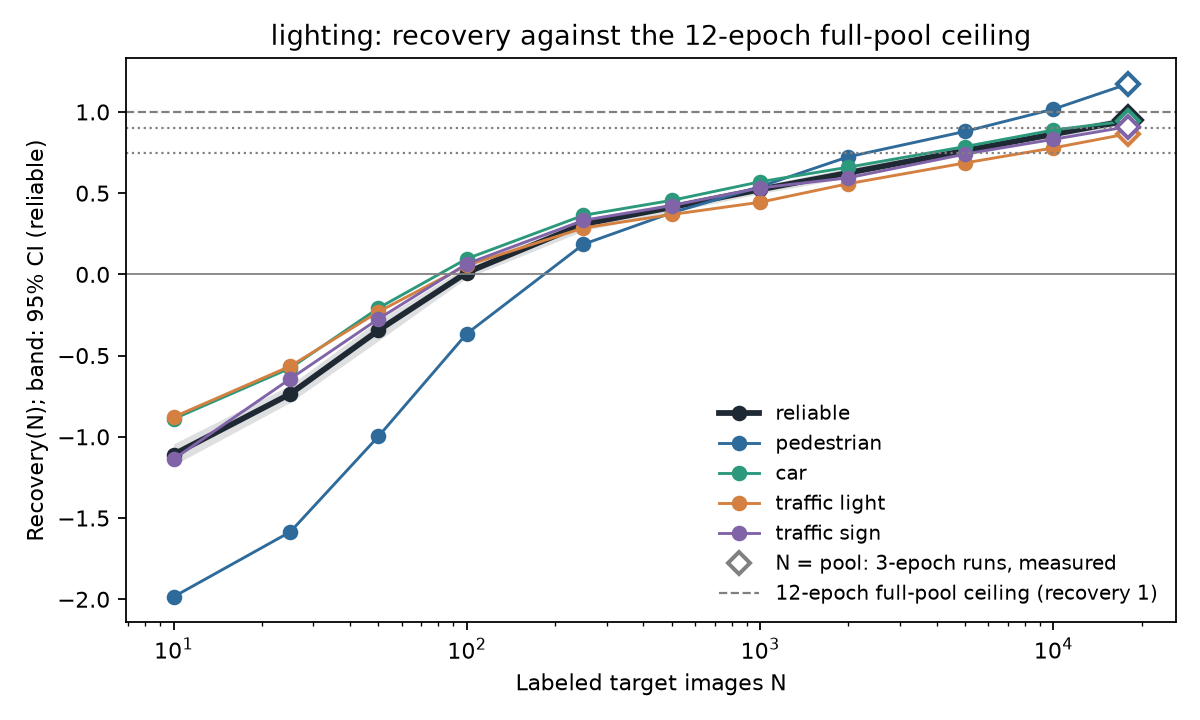
\includegraphics[width=\columnwidth]{recovery_lighting_e12.png}
\caption{Lighting: recovery against the 12-epoch ceiling. The last rung is the 3-epoch full-pool run, now a measurement (0.95).}
\label{fig:rec-lighting-e12}
\end{figure}

\begin{figure}[t]
\centering
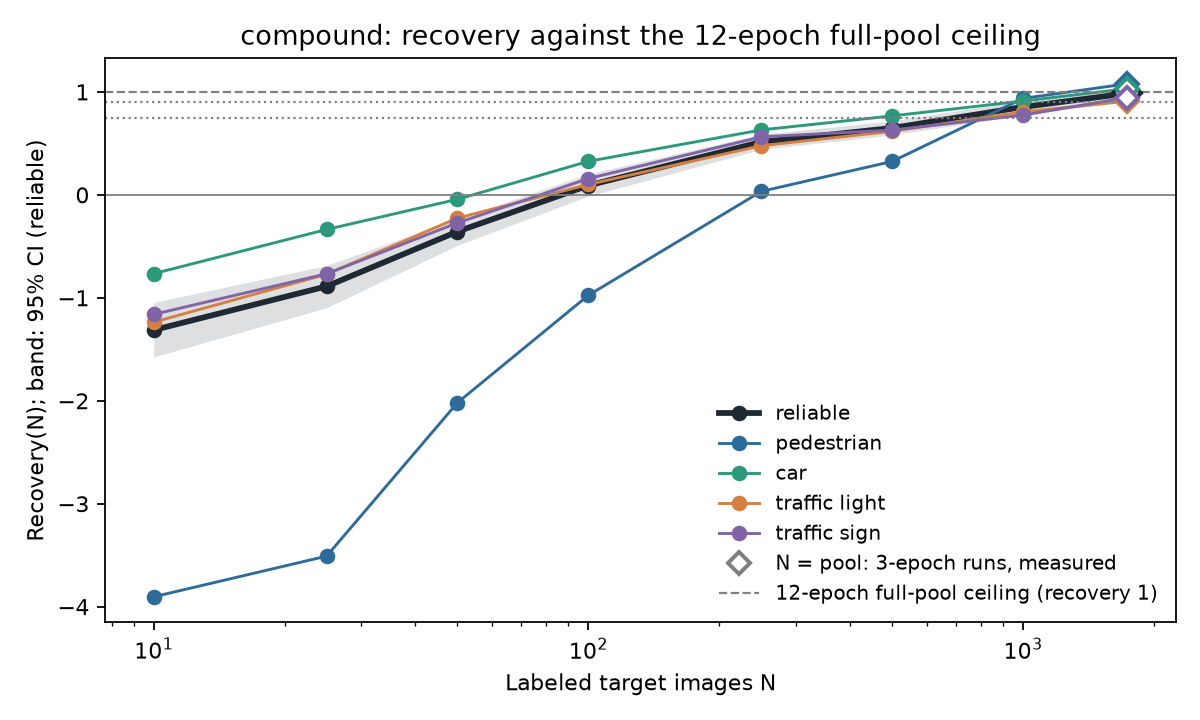
\includegraphics[width=\columnwidth]{recovery_compound_e12.png}
\caption{Compound: recovery against the 12-epoch ceiling. The last rung is the 3-epoch full-pool run (0.99).}
\label{fig:rec-compound-e12}
\end{figure}

Conclusion: \textbf{the 3-epoch ceiling is not materially undertrained relative to a schedule four times longer.} Twelve epochs add only 0.003 AP on the largest pool and nothing on the small pools. Note that the 12-epoch lighting ceiling, about 216,000 image passes, is still much shorter than the standard 1$\times$ schedule; this test rules out undertraining within the range of 3 to 12 epochs at the locked LR, but it does not rule out every possibility.

\section{Secondary Practical Result: Labeled-Budget Thresholds}\label{sec:thresholds}

\subsection{Thresholds against the Two Ceilings (RQ3)}\label{sec:thr-two}

\begin{table*}[t]
\centering
\caption{Thresholds \NBE, \Nsf, \Nnf (reliable mAP, full pool).}
\label{tab:thr}
\footnotesize
\setlength{\tabcolsep}{3pt}
\begin{tabular}{@{}llll@{}}
\toprule
Shift & Threshold & 3-epoch ceiling (CI range) & 12-epoch ceiling (CI range) \\
\midrule
lighting & \NBE & 100 (100--250) & 100 (100--250) \\
         & \Nsf & 5,000 (5,000) & 5,000 (5,000--10,000) \\
         & \Nnf & 10,000 (10,000--full pool) & full pool, 18,015 \\
\midrule
compound & \NBE & 100 (100--250) & 100 \\
         & \Nsf & 1,000 (1,000) & 1,000 \\
         & \Nnf & not determined within the pool ($>1{,}000$) & 1,738 (1,000--1,738) \\
\midrule
weather  & \NBE & 250 (250) & undetermined \\
         & \Nsf & 1,000 (1,000--full pool) & undetermined \\
         & \Nnf & not determined within the pool ($>1{,}000$) & undetermined \\
\bottomrule
\end{tabular}
\tabnote{With the 12-epoch ceiling, the ``full pool'' rung is the 3-epoch full-pool run, a real measurement. Each threshold is specific to the schedule $S = 500$, $E = 3$; it is not a property of the data alone.}
\end{table*}

\begin{itemize}
\item \textbf{Lighting:} \NBE is unchanged (Table~\ref{tab:thr}). \Nsf stays at the 5,000 rung, but only narrowly against the 12-epoch ceiling (recovery 0.76, CI 0.73--0.79). \Nnf moves from 10,000 up to the full pool, because recovery at $N = 10{,}000$ falls from 0.91 to 0.86.
\item \textbf{Compound:} \NBE and \Nsf are unchanged. \Nnf was previously not determined within the pool; with the 12-epoch ceiling, the 3-epoch full-pool rung reaches a recovery of 0.99, so $\Nnf = 1{,}738$.
\item \textbf{Weather is undetermined against the 12-epoch ceiling:} the denominator is only 0.011 AP, and 339 of the 1,000 bootstrap resamples of the recovery curve are undetermined. The 3-epoch full-pool run is even 0.0045 AP above the 12-epoch ceiling.
\item \textbf{Why \Nnf for weather and compound is not determined within the pool against the 3-epoch ceiling:} the largest rung actually measured is $N = 1{,}000$ (recovery 0.77 and 0.87); the next rung is the ceiling itself, equal to 1 by definition. The data only show that $\Nnf > 1{,}000$.
\item Three thresholds should be read with caution: weather $\Nsf = 1{,}000$ (recovery 0.77, lower CI bound 0.66); lighting $\Nnf = 10{,}000$ against the 3-epoch ceiling (lower CI bound 0.895); lighting $\NBE = 100$ (recovery $+0.01$, CI contains 0, a narrow break-even).
\end{itemize}

\subsection{Log-Linear Fit on the Positive Region}\label{sec:fit}

The fit is used only to interpolate between rungs. With the 3-epoch ceiling, all three shifts have a positive region starting at $N = 250$, but only lighting has at least 4 rungs (250--10,000, 6 rungs). With the 12-epoch ceiling, the 3-epoch full-pool rung belongs to the fit region, so compound reaches 4 rungs. The weather fit against the 12-epoch ceiling is not cited.

\begin{table*}[t]
\centering
\caption{Fit of $\mathrm{Recovery} = \alpha + \beta \cdot \ln N$ on the positive, monotonic region.}
\label{tab:fit}
\footnotesize
\setlength{\tabcolsep}{3pt}
\begin{tabular}{@{}lllccc@{}}
\toprule
Shift & Ceiling & Fit region & $R^2$ & \Nsf from fit (95\% CI) & \Nnf from fit (95\% CI) \\
\midrule
lighting & 3 epochs  & 250--10,000, 6 rungs & 0.9999 & 3,570 (3,250--3,960) & 9,200 (8,280 to $>10{,}000$) \\
lighting & 12 epochs & 250--18,015, 7 rungs & 0.9999 & 4,690 (4,070--5,340) & 12,800 (10,870--14,970) \\
compound & 12 epochs & 250--1,738, 4 rungs  & 0.9937 & 680 (530--880)       & 1,240 (980--1,630) \\
\bottomrule
\end{tabular}
\end{table*}

\begin{itemize}
\item Lighting (Table~\ref{tab:fit}): \Nsf lies in the range 3,570--4,690 images and \Nnf in the range 9,200--12,800 images, depending on the ceiling. The threshold against the 3-epoch ceiling is a lower bound and the one against the 12-epoch ceiling is an upper bound, because the large rungs of the ladder are trained for only 3 epochs. Both fall within the corresponding ladder interval; the ladder interval remains the main result.
\item A high $R^2$ on the fit region is not strong evidence, because the region has only 4--7 points that are nearly collinear in $\ln N$. A more meaningful test is a held-out check: a fit on the three lighting rungs 250, 500 and 1,000 predicts 0.663 / 0.812 / 0.924 at $N = 2{,}000$ / $5{,}000$ / $10{,}000$, against measured values of 0.660 / 0.804 / 0.911 (3-epoch ceiling). The error grows with $N$ ($+0.003$, $+0.008$, $+0.013$), so the fit is slightly optimistic when extrapolating.
\item Sensitivity to the choice of region: if the region starts at the point estimate of \NBE ($N = 100$), the lighting $R^2$ drops to 0.973 with the 3-epoch ceiling; the $N = 100$ rung is not yet in the log-linear region.
\item The full-pool point lies almost exactly on the log-linear line of the smaller rungs (predicted 1.007 against the 3-epoch ceiling): according to the data, the lighting curve has not saturated.
\end{itemize}

\subsection{Weather in Raw AP}\label{sec:weather-raw}

Table~\ref{tab:weatherap} gives the weather reliable mAP at each rung and its change from zero-shot.

\begin{table}[t]
\centering
\caption{Weather: reliable mAP by $N$ (seed mean; zero-shot 0.3201).}
\label{tab:weatherap}
\footnotesize
\setlength{\tabcolsep}{3pt}
\begin{tabular}{@{}lcl@{}}
\toprule
$N$ & mAP & vs.\ zero-shot (95\% CI) \\
\midrule
10    & 0.2659 & $-$0.0542 ($-$0.0641, $-$0.0443) \\
25    & 0.2852 & $-$0.0349 \\
50    & 0.2986 & $-$0.0215 \\
100   & 0.3136 & $-$0.0065 ($-$0.0118, $-$0.0017) \\
250   & 0.3236 & $+$0.0035 \\
500   & 0.3279 & $+$0.0078 \\
1,000 & 0.3319 & $+$0.0118 ($+$0.0088, $+$0.0142) \\
full pool, 3 epochs  & 0.3355 & $+$0.0154 \\
full pool, 12 epochs & 0.3310 & $+$0.0109 \\
\bottomrule
\end{tabular}
\tabnote{CIs are available only for the three rungs computed in the RQ5 analysis. The $N = 1{,}000$ rung is already on par with the 12-epoch ceiling.}
\end{table}

\subsection{Comparison across Shifts at the Same Pool Size (RQ4)}\label{sec:rq4}

\begin{table*}[t]
\centering
\caption{Pool of 1,738 images, 3-epoch ceiling (2 seeds per shift).}
\label{tab:rq4}
\footnotesize
\setlength{\tabcolsep}{3pt}
\begin{tabular}{@{}lcccl@{}}
\toprule
Shift & Recovery, $N = 500$ (95\% CI) & Recovery, $N = 1{,}000$ (95\% CI) & \Nsf & \Nnf \\
\midrule
lighting & 0.67 (0.63, 0.72) & 0.85 (0.81, 0.90) & 1,000 & not determined within the pool ($>1{,}000$) \\
weather  & 0.54 (0.42, 0.65) & 0.82 (0.71, 0.92) & 1,000 (1,000--1,738) & not determined within the pool ($>1{,}000$) \\
compound & 0.66 (0.61, 0.71) & 0.87 (0.82, 0.91) & 1,000 & not determined within the pool ($>1{,}000$) \\
\bottomrule
\end{tabular}
\end{table*}

At the same pool size (Table~\ref{tab:rq4}), lighting and compound recover at almost the same rate; weather is slower at $N = 500$ but catches up at $N = 1{,}000$, and all three have $\Nsf = 1{,}000$. The differences between shifts in Section~\ref{sec:thr-two} therefore come mainly from the magnitude of the ceiling and the pool size, not from the speed of learning. Against the 12-epoch ceiling on the 1,738-image pool: lighting has $\Nsf = \Nnf = 1{,}000$ (recovery 0.91, CI 0.84--0.97), compound has $\Nsf = 1{,}000$ and $\Nnf = 1{,}738$, and weather is undetermined (denominator 0.0099 AP).
